\chapter{Introduction}
The Ada Crypto Lib (ACL) is a free cryptographic library written in Ada.
One of the two main design objectives of this library is to create
an \textbf{intuitive and clean API}. The other goal is to use a clean
programming style in order to actively support and simplify formal code
verification. Due to this, the ACL has been coded without the
following "features":
\begin{itemize}
\item inline assembler
\item tagged types (objects)
\item goto statements
\end{itemize}

Goto statements have been avoided as they make the source more complex
and might cause problems during formal verification of the code. No
tagged types have been used as procedures and methods may be
overwritten, and the actual method that is being utilised is
determined during runtime (dynamic dispatching). This results in
massive problems during formal code verification. Inline assembler has
been avoided cause it involves a very unclean programming style and
can be used for omitting the strict typing of Ada. Due to these
restrictions, the actual code quality increases with respect to
verification and security, however they also lead to decreased
performance.  If you favor performance over clean design, you should
possibly look for another cryptographic library. Unfortunately, there
are currently no other free cryptographic libraries for Ada we can
refer to.

The ACL is in the status of a "proof of concept". There might be the
possibility that sensible materials, such as the key, might still be
resident within the RAM after a program using the ACL has been
terminated. A storage pool dealing with this restriction is currently
being developed. Most of the other cryptographic libraries that share
this limitation do not inform about the possible weakness. Those
libraries should not be used as they can not be considered reliable.

The following subsumes the disadvantages of the ACL:
\begin{itemize}
\item missing cleanup of stack and heap
\item no "big-endian" support
\item bad performance
\end{itemize}

This documentation subsumes briefly the installation and the
topological structure.  Then it solely describes the API. Each package
and its API are introduced in a separate chapter. Each chapter
concludes with one or more examples.

If you have any questions about the ACL, encounter a bug or want to
contribute one or several packages, feel free to contact us via email:
cforler@gmx.de.

%%%%%%%%%%%%%%%%%%%%%%%%%%%%%%%%%%%%%%%%%%%%%%%%%%%%%%%%%%%%%%%%%%%%%%%%%%%

\section{Installation HOWTO}
On a Linux system, the following packages are required to install the ACL:
\begin{itemize}
\item \texttt{gnat}
\item \texttt{make}
\item \texttt{binutils}
\item \texttt{git}
\item \texttt{GCOV, LCOV (optional)}
\end{itemize}

\subsubsection{Compilation}
The following commands can be used to get and compile the ACL as
well as the regression test included. \bigskip
\begin{lstlisting}[style=BashInputStyle]
    # git clone git://github.com/cforler/Ada-Crypto-Library.git
    # cd Ada-Crypto-Library
    # make
    # make acltest
\end{lstlisting}

\subsubsection{Testing}
Before you actually install the ACL you should run the regression test
in order to make sure the ACL properly works on your computer
system. The following command sequence can be used to run the
regression test.\bigskip
\begin{lstlisting}[style=BashInputStyle]
    # cd test
    # ./test-tests
    # cd ..
\end{lstlisting}
Since the total regression test may last a few minutes, the tests are
additionally divided into five main categories, which can be run
seperately (Figure \ref{ACLTEST}): \texttt{Test-Big\_Number},
\texttt{Test-Symmetric\_Ciphers}, \texttt{Test-Asymmetric\_Ciphers},
\texttt{Test-Hash} and \texttt{Test-MISC}.

\subsubsection{Installation and De-installation}
If no errors were encountered during the regression test, the ACL can
be installed by issuing the following command:\bigskip
\begin{lstlisting}[style=BashInputStyle]
    # sudo make install
\end{lstlisting}
The following command can be used to remove the ACL:\bigskip
\begin{lstlisting}[style=BashInputStyle]
    # sudo make uninstall
\end{lstlisting}

\subsubsection{Recompilation}
The following commands can be used to recompile the ACL:\bigskip
\begin{lstlisting}[style=BashInputStyle]
    # make clean
    # make
    # make acltest
\end{lstlisting}

\subsubsection{Installiation and De-installation -Shared Library}
The ACL may be installed as a shared library (libacl.so) with the
following commands:\bigskip
\begin{lstlisting}[style=BashInputStyle]
    # make shared
    # make install-shared
\end{lstlisting}
The shared library can be de-installed with the following command:\bigskip
\begin{lstlisting}[style=BashInputStyle]
    # sudo make uninstall-shared
\end{lstlisting}

\subsubsection{Documentation}
The tetex-bin (latex) and the tetex-extra packages are needed to
install this documentation. The complete ACL documentation (german \&
english) can be generated with the following command:\bigskip
\begin{lstlisting}[style=BashInputStyle]
    # make doc
\end{lstlisting}
The documentation will be copied to
\texttt{/usr/local/share/doc/libadacrypt-dev} with the following command:\bigskip
\begin{lstlisting}[style=BashInputStyle]
    # sudo make install-doc
\end{lstlisting}
The documentation in \texttt{/usr/local/share/doc/libadacrypt-dev} can
be uninstalled with the following command:\bigskip
\begin{lstlisting}[style=BashInputStyle]
    # sudo make uninstall-doc
\end{lstlisting}

\subsubsection{Adaptations}
The \texttt{Makefiles} can be found in the \texttt{src} directory. It can be used to
adapt the following variables:
\begin{itemize}
\item LIBDIR : installation path for the shared library.
\item INSTDIR : installation path for the ACL.
\end{itemize}

%%%%%%%%%%%%%%%%%%%%%%%%%%%%%%%%%%%%%%%%%%%%%%%%%%%%%%%%%%%%%%%%%%%%%%%%%%%

\section{Directories and Package Layout}
\subsubsection{Directories}
\begin{itemize}
\item doc : documentation
\item ref : references and specifications
\item src : source code
\item test : regression test
\end{itemize}

%%%%%%%%%%%%%%%%%%%%%%%%%%%%%%%%%%%%%%%%%%%%%%%%%%%%%%%%%%%%%%%%%%%%%%%%%%%

\subsubsection{Package Layout}
Figure \ref{Layout_of_ACL} shows the composed packages of the ACL.
\begin{figure}[h]
  \centering
  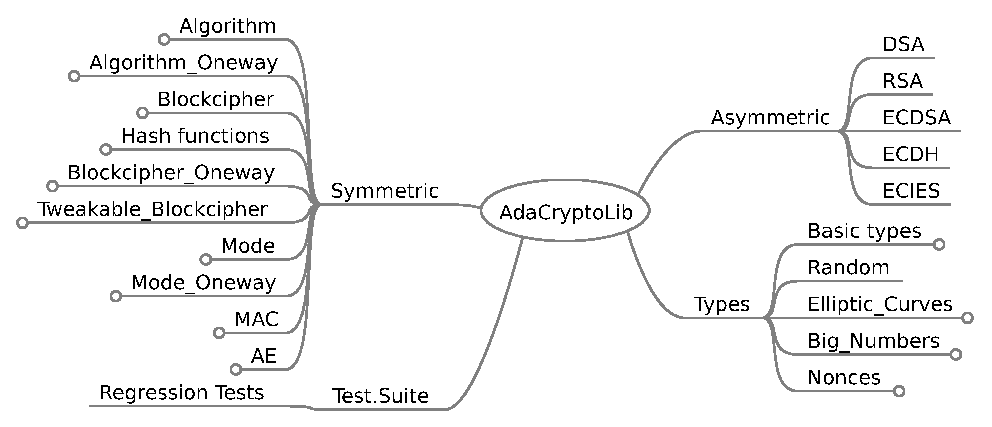
\includegraphics[scale=0.9]{./images/Layout_of_the_ACL}
  \caption{Layout of the ACL.} \label{Layout_of_ACL}
\end{figure}
\begin{description}
\item[Crypto:]\ \\
  It is the root package of the ACL. All other ACL packages start with the prefix \texttt{Crypto}.
\item[Crypto.Types:] \ \\
  Fundamental and derived types (such as bytes and blocks) with their corresponding functionalities are in this package. Utilization of the ACL is very limited without including this package.
\item[Crypto.Types.Random:] \ \\
  It provides an interface between an external random bit generator and the ACL.
\item[Crypto.Types.Elliptic\_Curves:] \ \\
  This package provides types based on the rules of elliptic curves.
\item[Crypro.Types.Big\_Numbers:] \ \\
  This package provides a generic type, whose length is a multiple of 32 bits.
\item[Crypto.Types.Nonces:] \ \\
  This package is used to provide nonce (number used once) values.
\item[Crypto.Symmetric:]\ \\
  This is the root package of the symmetric branch.
\item[Crypto.Symmetric.Algorithm:]\ \\
  This package contains the symmetric algorithms for blockciphers and hashfunctions.
\item[Crypto.Symmetric.Algorithm.Oneway:]\ \\
  Each algorithm has an one-way algorithm, which is contained in this package. 
\item[Crypto.Symmetric.Blockcipher:]\ \\
  This generic package is used to generate a blockcipher from a symmetric algorithm.
\item[Crypto.Symmetric.Oneway\_Blockcipher:]\ \\
  This package can be used to generate a one-way blockcipher from a
  symmetric one-way algorithm.
\item[Crypto.Symmetric.Tweakable\_Blockcipher:] \ \\
  This kind of blockcipher serves by using a tweak value.
\item[Crypto.Symmetric.Hashfunction:] \ \\
  It is used to generate a hash function building block.
\item[Crypto.Symmetric.Mode:]\ \\
  This package contains several modes of operation based on blockciphers.
\item[Crypto.Symmetric.Mode.Oneway:]\ \\
  This package contains several modes of operation based on one-way blockciphers.
\item[Crypto.Symmetric.MAC:] \ \\
  This package provides MAC (Message Authentication Code) operations.
\item[Crypto.Symmetric.AE:] \ \\
  This package provides AE (Authenticated Encryption) schemes.
\item[Crypto.Asymmetric:]\ \\
  This is the root package of the asymmetric branch.
\item[Crypto.Asymmetric.RSA:]\ \\
  This package provides the RSA algorithm.
\item[Crypto.Asymmetric.DSA:]\ \\
  This package contains the DSA (Digital Signature Algorithm) algorithm.
\item[Crypto.Asymmetric.ECDSA:]\ \\
  This package provides the elliptic curve DSA algorithm.
  \item[Crypto.Asymmetric.ECDH:]\ \\
  This package provides the ECDH (Elliptic Curve Diffie–Hellman) algorithm.
\item[Crypto.Asymmetric.ECIES:]\ \\
  This package provides the ECIES (Elliptic Curve Integrated Encryption Scheme) algorithm.
\item[Crypto.Test.Suite:]\ \\
  This package contains the regression test for the ACL.
\end{description}
